\documentclass[aspectratio=169,11pt]{beamer}

\def\courseTitle{Industrial Security (Bachelor)}
\def\courseSubtitle{Section 04 -- Industrial Protocols}
\def\sectionNumber{04}
\def\sectionTitle{Industrial Protocols}

% =====================================================================
% Industrial Security lecture series -- modern Beamer preamble.
%
% Each slide deck must define the following BEFORE \input{}-ing this:
%   \def\courseTitle{...}        e.g. Industrial Security (Bachelor)
%   \def\courseSubtitle{...}     e.g. Section 3 -- Network Architecture
%   \def\sectionNumber{...}      e.g. 03
%   \def\sectionTitle{...}       e.g. Industrial Network Architectures
%
% Optional:
%   \def\courseAuthor{...}       defaults to "Lecture Notes"
%   \def\courseInstitute{...}    defaults to "Department of Computer Science"
%   \def\companyLogo{...}        path to a logo image (PDF/PNG/JPG).
%
% Callout macros (use anywhere inside a frame):
%   \begin{notebox}{title}      ... \end{notebox}
%   \begin{importantbox}{title} ... \end{importantbox}
%   \begin{warningbox}{title}   ... \end{warningbox}
%   \begin{tipbox}{title}       ... \end{tipbox}
%   \begin{defbox}{title}       ... \end{defbox}
%   \begin{takeawaybox}{title}  ... \end{takeawaybox}
%   \begin{quotebox}            ... \end{quotebox}
% =====================================================================

% --- Speaker-notes mode (toggled by Makefile via -usepretex) ----------
% When notesmode=1, build a side-by-side slide+notes PDF for the
% lecturer. When unset/0, build the clean slides-only PDF.
\providecommand{\notesmode}{0}
\ifnum\notesmode=1
  \usepackage{pgfpages}
  \setbeameroption{show notes on second screen=right}
  \setbeamerfont{note page}{size=\small}
\fi

\usepackage[utf8]{inputenc}
\usepackage[T1]{fontenc}
\usepackage[english]{babel}
% Modern type pair: IBM Plex Sans for text, IBM Plex Mono for code.
% Math stays in lmodern; Plex is the dominant family on every text frame.
\usepackage{plex-sans}
\usepackage{plex-mono}
\renewcommand{\familydefault}{\sfdefault}
\usepackage[activate={true,nocompatibility},final,tracking=true,kerning=true,spacing=true,factor=1100,stretch=10,shrink=10]{microtype}
\usepackage{graphicx}
\usepackage{listings}
\usepackage{xcolor}
\usepackage{colortbl}
\usepackage{tikz}
\usepackage{booktabs}
\usepackage{array}
\usepackage{hyperref}
\usepackage{amsmath}
\usepackage{amssymb}
\usepackage{tcolorbox}
\tcbuselibrary{skins, breakable, raster}
\usepackage{fontawesome5}

% =====================================================================
% Shared TikZ styles for the Industrial Security lecture series.
% Loaded by every slide deck and exercise sheet that uses TikZ.
% =====================================================================

\usetikzlibrary{
  arrows.meta,
  shapes,
  shapes.geometric,
  shapes.symbols,
  shapes.multipart,
  positioning,
  fit,
  calc,
  backgrounds,
  decorations.pathmorphing,
  decorations.pathreplacing,
  decorations.text,
  patterns,
  matrix,
  shadows
}

% --- colour palette --------------------------------------------------
\definecolor{isOT}{HTML}{1F4E79}     % OT (deep blue)
\definecolor{isIT}{HTML}{6F2DA8}     % IT (purple)
\definecolor{isSafety}{HTML}{C00000} % safety red
\definecolor{isNet}{HTML}{2E7D32}    % network green
\definecolor{isAttack}{HTML}{B23A48} % attack red
\definecolor{isAccent}{HTML}{E08E0B} % amber
\definecolor{isMute}{HTML}{6B6B6B}   % grey
\definecolor{isLight}{HTML}{EDF2F8}  % light background
\definecolor{isPLC}{HTML}{2C5282}
\definecolor{isHMI}{HTML}{2F855A}
\definecolor{isSCADA}{HTML}{6B46C1}

% --- generic node styles --------------------------------------------
\tikzset{
  isnode/.style={
    draw, rounded corners=2pt, minimum height=8mm, minimum width=18mm,
    font=\small, align=center, thick
  },
  isbox/.style={isnode, fill=isLight},
  plc/.style={isnode, fill=isPLC!15, draw=isPLC, thick},
  hmi/.style={isnode, fill=isHMI!15, draw=isHMI, thick},
  scada/.style={isnode, fill=isSCADA!15, draw=isSCADA, thick},
  sensor/.style={isnode, fill=isNet!10, draw=isNet, minimum height=6mm, minimum width=14mm, font=\scriptsize},
  actuator/.style={isnode, fill=isAccent!15, draw=isAccent, minimum height=6mm, minimum width=14mm, font=\scriptsize},
  firewall/.style={isnode, fill=isAttack!15, draw=isAttack, thick},
  server/.style={isnode, fill=isMute!15, draw=isMute!80, thick},
  switch/.style={isnode, fill=isLight, draw=black!60, minimum height=6mm, minimum width=14mm, font=\scriptsize},
  workstation/.style={isnode, fill=white, draw=isOT, thick},
  attacker/.style={isnode, fill=isAttack!20, draw=isAttack, thick, font=\small\bfseries},
  inetnode/.style={draw, ellipse, minimum width=24mm, minimum height=10mm, font=\scriptsize, fill=isLight, thick},
  process/.style={isnode, fill=isOT!15, draw=isOT, thick, minimum width=24mm},
  zone/.style={
    draw, rounded corners=4pt, thick, dashed, inner sep=4mm
  },
  conduit/.style={-{Stealth[length=2.5mm]}, thick, isNet!80!black},
  attack/.style={-{Stealth[length=2.5mm]}, thick, isAttack, dashed},
  flow/.style={-{Stealth[length=2.5mm]}, thick, isOT!70!black},
  netline/.style={thick, black!60},
  axisline/.style={-{Stealth[length=2mm]}, thick, black!70},
  tag/.style={font=\scriptsize\itshape, fill=white, inner sep=1pt},
  level/.style={
    draw, fill=isLight, minimum width=0.85\linewidth, minimum height=8mm,
    font=\small, anchor=west
  },
  brace/.style={decorate, decoration={brace, amplitude=4pt, raise=2pt}},
  legendbox/.style={draw, rounded corners=2pt, fill=isLight, inner sep=2mm, font=\scriptsize, align=left}
}

% --- handy macros ----------------------------------------------------
% \plcicon, \hmiicon etc as simple labelled boxes; useful inline.
\newcommand{\plcicon}[1][PLC]{\tikz[baseline=-0.6ex]{\node[plc, minimum width=10mm, minimum height=5mm, font=\scriptsize, inner sep=1pt]{#1};}}
\newcommand{\hmiicon}[1][HMI]{\tikz[baseline=-0.6ex]{\node[hmi, minimum width=10mm, minimum height=5mm, font=\scriptsize, inner sep=1pt]{#1};}}
\newcommand{\fwicon}[1][FW]{\tikz[baseline=-0.6ex]{\node[firewall, minimum width=10mm, minimum height=5mm, font=\scriptsize, inner sep=1pt]{#1};}}


\graphicspath{{.}{../../../template/}}

% --- defaults --------------------------------------------------------
\providecommand{\courseAuthor}{Lecture Notes}
\providecommand{\courseInstitute}{Department of Computer Science}
\providecommand{\companyLogo}{logo}

% --- modern palette --------------------------------------------------
\definecolor{slideAccent}{HTML}{1F4E79}       % primary navy
\definecolor{slideSecondary}{HTML}{E08E0B}    % amber accent

% --- Corporate branding overrides ------------------------------------
% A user-editable `branding.tex` at the repo root can override the
% logo path, author/institute lines, and brand colours. If the file is
% missing the built-in defaults above stay in effect.
\IfFileExists{../../../branding.tex}{% =====================================================================
% Corporate / institutional branding -- single file to customise the
% look of the entire course (slides, notes, exercises, labs).
%
% HOW TO REBRAND IN UNDER A MINUTE:
%   1. Replace `branding/logo.pdf` with your own logo
%      (PDF preferred; PNG and JPG also work -- name it `logo.<ext>`).
%   2. (Optional) change the two colours below to your brand palette.
%   3. (Optional) override the author/institute lines below.
%   4. Re-run `make` at the repo root. That's it.
%
% Everything in this file has sensible defaults; you can delete a line
% to fall back to the built-in defaults, or comment it out.
%
% This file is loaded automatically by the slides, exercise, and lab
% preambles -- you never need to \input it manually.
% =====================================================================

% --- Logo --------------------------------------------------------------
% Path is resolved from each leaf-build directory; the default points at
% the shared `branding/` folder at the repo root. If you put your logo
% somewhere else, set the full or relative path here (without extension):
\renewcommand{\companyLogo}{../../../branding/logo}

% --- Author / institute (appears on the title page footer) ------------
\renewcommand{\courseAuthor}{}
\renewcommand{\courseInstitute}{}

% --- Brand colours ----------------------------------------------------
% slideAccent      = primary brand colour (title bands, accent rule)
% slideSecondary   = secondary brand colour (section badge, highlight)
% Both use HTML hex codes. Keep enough contrast against white text.
\definecolor{slideAccent}{HTML}{00205B}      % deep navy
\definecolor{slideSecondary}{HTML}{00A0DC}   % light blue accent
}{}
\definecolor{slideTitle}{HTML}{0F2A44}        % near-black navy
\definecolor{slideMuted}{HTML}{6B6B6B}
\definecolor{slideBg}{HTML}{FFFFFF}
\definecolor{slidePanel}{HTML}{F4F7FB}
\definecolor{slideRule}{HTML}{D6DEE8}

% Callout colours
\definecolor{calNote}{HTML}{1F4E79}
\definecolor{calImportant}{HTML}{B23A48}
\definecolor{calWarning}{HTML}{C77700}
\definecolor{calTip}{HTML}{2E7D32}
\definecolor{calDef}{HTML}{6B46C1}
\definecolor{calTake}{HTML}{0F2A44}

% --- beamer theme ---------------------------------------------------
\useinnertheme{rectangles}
\usefonttheme{professionalfonts}

\setbeamertemplate{navigation symbols}{}
\setbeamertemplate{itemize items}[circle]
\setbeamertemplate{enumerate items}[default]
\setbeamertemplate{section in toc}[ball numbered]
\setbeamercolor{section in toc}{fg=slideTitle}

% Colours
\setbeamercolor{normal text}{fg=slideTitle, bg=slideBg}
\setbeamercolor{title}{fg=slideAccent}
\setbeamercolor{subtitle}{fg=slideMuted}
\setbeamercolor{frametitle}{fg=slideAccent}
\setbeamercolor{structure}{fg=slideAccent}
\setbeamercolor{itemize item}{fg=slideAccent}
\setbeamercolor{itemize subitem}{fg=slideSecondary}
\setbeamercolor{block title}{fg=white, bg=slideAccent}
\setbeamercolor{block body}{fg=slideTitle, bg=slidePanel}
\setbeamercolor{alerted text}{fg=slideSecondary}

% Fonts
\setbeamerfont{title}{series=\bfseries, size=\Large}
\setbeamerfont{subtitle}{series=\mdseries, size=\normalsize}
\setbeamerfont{frametitle}{series=\bfseries, size=\large}
\setbeamerfont{block title}{series=\bfseries, size=\normalsize}
\setbeamerfont{footline}{size=\tiny}

% --- frametitle: title bar + accent underline + section badge -------
% The accent rules are wrapped in a zero-width box so they never
% contribute to the surrounding hbox width (no Overfull warnings).
\setbeamertemplate{frametitle}{%
  \nointerlineskip
  \begin{beamercolorbox}[wd=\paperwidth, ht=2.8ex, dp=1.6ex, leftskip=1.2em, rightskip=1.2em]{frametitle}%
    \usebeamerfont{frametitle}\insertframetitle%
    \hfill
    {\color{slideMuted}\small \sectionNumber}%
  \end{beamercolorbox}%
  \nointerlineskip
  \makebox[0pt][l]{\hspace*{1.2em}\textcolor{slideSecondary}{\rule{2.5em}{1pt}}\textcolor{slideAccent}{\rule{\dimexpr\paperwidth-3.7em\relax}{1pt}}}%
  \par\vskip4pt
}

% --- footer ---------------------------------------------------------
\defbeamertemplate*{footline}{is-footer}{%
  \leavevmode%
  \hbox{%
    \begin{beamercolorbox}[wd=.55\paperwidth, ht=2.4ex, dp=1ex, leftskip=1em]{author in head/foot}%
      {\color{slideMuted}\tiny \courseTitle{} \;\; $\bullet$ \;\; Section \sectionNumber{} -- \sectionTitle}%
    \end{beamercolorbox}%
    \begin{beamercolorbox}[wd=.45\paperwidth, ht=2.4ex, dp=1ex, rightskip=1em]{title in head/foot}%
      \hfill {\color{slideMuted}\tiny \insertframenumber{} / \inserttotalframenumber}%
    \end{beamercolorbox}%
  }%
  \vskip2pt
}

% --- listings -------------------------------------------------------
\definecolor{codebg}{HTML}{F4F7FB}
\definecolor{codekw}{HTML}{0F2A44}
\definecolor{codestr}{HTML}{8B3A3A}
\definecolor{codecom}{HTML}{5A7D54}

\lstset{
    backgroundcolor=\color{codebg},
    basicstyle=\ttfamily\scriptsize\color{slideTitle},
    keywordstyle=\color{codekw}\bfseries,
    stringstyle=\color{codestr},
    commentstyle=\color{codecom}\itshape,
    breaklines=true,
    frame=leftline,
    framerule=2pt,
    rulecolor=\color{slideAccent},
    numbers=left,
    numberstyle=\tiny\color{slideMuted},
    numbersep=8pt,
    showstringspaces=false,
    tabsize=2,
    captionpos=b,
    xleftmargin=0.6em
}

% --- callout boxes --------------------------------------------------
% Shared base style for all callout boxes.
% Subtle drop shadow gives the boxes a hint of elevation without distraction.
\tcbset{
  isCallout/.style={
    enhanced, breakable, sharp corners=northeast,
    arc=2pt, boxrule=0pt,
    leftrule=3pt,
    fonttitle=\bfseries\small,
    coltitle=white,
    fontupper=\small,
    left=2mm, right=2mm, top=1.5mm, bottom=1.5mm,
    drop fuzzy shadow=black!30,
    title={#1}
  }
}

\newtcolorbox{notebox}[1]{
  isCallout={#1},
  colback=calNote!8, colframe=calNote, leftrule=3pt,
  colbacktitle=calNote, attach boxed title to top left={xshift=2mm, yshift=-1.2mm},
  boxed title style={colback=calNote, arc=1pt, boxrule=0pt, left=2mm, right=2mm, top=0.5mm, bottom=0.5mm}
}

\newtcolorbox{importantbox}[1]{
  isCallout={#1},
  colback=calImportant!7, colframe=calImportant, leftrule=4pt,
  colbacktitle=calImportant, attach boxed title to top left={xshift=2mm, yshift=-1.2mm},
  boxed title style={colback=calImportant, arc=1pt, boxrule=0pt, left=2mm, right=2mm, top=0.5mm, bottom=0.5mm}
}

\newtcolorbox{warningbox}[1]{
  isCallout={#1},
  colback=calWarning!10, colframe=calWarning, leftrule=4pt,
  colbacktitle=calWarning, attach boxed title to top left={xshift=2mm, yshift=-1.2mm},
  boxed title style={colback=calWarning, arc=1pt, boxrule=0pt, left=2mm, right=2mm, top=0.5mm, bottom=0.5mm}
}

% Alias warnbox = warningbox, with an optional title (default = "Caution")
\newtcolorbox{warnbox}[1][Caution]{
  isCallout={#1},
  colback=calWarning!10, colframe=calWarning, leftrule=4pt,
  colbacktitle=calWarning, attach boxed title to top left={xshift=2mm, yshift=-1.2mm},
  boxed title style={colback=calWarning, arc=1pt, boxrule=0pt, left=2mm, right=2mm, top=0.5mm, bottom=0.5mm}
}

\newtcolorbox{tipbox}[1]{
  isCallout={#1},
  colback=calTip!8, colframe=calTip, leftrule=3pt,
  colbacktitle=calTip, attach boxed title to top left={xshift=2mm, yshift=-1.2mm},
  boxed title style={colback=calTip, arc=1pt, boxrule=0pt, left=2mm, right=2mm, top=0.5mm, bottom=0.5mm}
}

\newtcolorbox{defbox}[1]{
  isCallout={#1},
  colback=calDef!8, colframe=calDef, leftrule=3pt,
  colbacktitle=calDef, attach boxed title to top left={xshift=2mm, yshift=-1.2mm},
  boxed title style={colback=calDef, arc=1pt, boxrule=0pt, left=2mm, right=2mm, top=0.5mm, bottom=0.5mm}
}

\newtcolorbox{takeawaybox}[1]{
  enhanced, breakable, arc=3pt, boxrule=0pt,
  colback=calTake!7, colframe=calTake,
  toptitle=2mm, bottomtitle=2mm,
  fonttitle=\bfseries\normalsize, coltitle=white,
  colbacktitle=calTake,
  fontupper=\small,
  title={\faStar~Key Takeaway: #1},
  left=3mm, right=3mm, top=2mm, bottom=2mm
}

\newtcolorbox{quotebox}{
  enhanced, breakable, arc=2pt, boxrule=0pt,
  colback=slidePanel, colframe=slideMuted,
  leftrule=3pt, top=2mm, bottom=2mm, left=3mm, right=3mm,
  fontupper=\itshape\small,
}

% Convenience: inline highlight badge
\newcommand{\remembertag}{\tikz[baseline=-0.7ex]\node[fill=calImportant, text=white, font=\scriptsize\bfseries, rounded corners=2pt, inner sep=2pt]{REMEMBER};}
\newcommand{\tldr}{\tikz[baseline=-0.7ex]\node[fill=calTake, text=white, font=\scriptsize\bfseries, rounded corners=2pt, inner sep=2pt]{TL;DR};}

% Source attribution: tiny grey line, anchored bottom-left of the content area
% Usage:  \source{Symantec, \emph{W32.Stuxnet Dossier} v1.4, 2011.}
% Multiple sources:  \source{X.\ Y., 2018; Z, 2020.}
\newcommand{\source}[1]{%
  \par\nointerlineskip\vspace{0.4mm}%
  {\color{slideMuted}\fontsize{5.5}{6.5}\selectfont\textit{Source:} #1\par}%
}

% References slide: aggregate citations + further reading at the end of a section.
% Usage:  \referencesframe{ \item ... \item ... }
% The `frame` environment must be written literally in the deck, so this is a
% macro rather than a wrapper environment (beamer collects the frame body and
% trips over \newenvironment wrappers).
%
% allowframebreakstemplate=\insertcontinuationcount silences the trailing roman
% numeral when content fits on a single page.
\setbeamertemplate{frametitle continuation}[from second]
\newcommand{\referencesframe}[1]{%
  \begin{frame}[allowframebreaks]{References -- Section \sectionNumber}
    \fontsize{7.5}{9}\selectfont
    \setlength{\itemsep}{1pt}
    \begin{itemize}#1\end{itemize}
  \end{frame}%
}

% --- title page -----------------------------------------------------
\title[\courseTitle]{\courseTitle}
\subtitle{\courseSubtitle}
\author{\courseAuthor}
\institute{\courseInstitute}
\date{}

% Logo lookup: try the section directory, then the shared template/.
\newcommand{\showlogo}[1][2cm]{%
  \IfFileExists{\companyLogo.pdf}{\includegraphics[width=#1]{\companyLogo}}{%
    \IfFileExists{\companyLogo.png}{\includegraphics[width=#1]{\companyLogo}}{%
      \IfFileExists{\companyLogo.jpg}{\includegraphics[width=#1]{\companyLogo}}{%
        \IfFileExists{../../../template/\companyLogo.pdf}{\includegraphics[width=#1]{../../../template/\companyLogo}}{%
          \rule{0pt}{0pt}}}}}}

\setbeamertemplate{title page}{%
  
\begin{tikzpicture}[remember picture, overlay]
    % accent band (taller to fit wrapped titles)
    \fill[slideAccent] (current page.north west) rectangle ([yshift=-3.4cm]current page.north east);
    \fill[slideSecondary] ([yshift=-3.4cm]current page.north west) rectangle ([yshift=-3.55cm]current page.north east);
    % section badge
    \node[fill=slideSecondary, text=white, font=\bfseries\normalsize, rounded corners=3pt, inner sep=4pt, anchor=north west]
      at ([xshift=1.2cm, yshift=-0.7cm]current page.north west) {Section \sectionNumber};
    % Course title (wraps if long)
    \node[anchor=north west, text=white, font=\bfseries\Large, align=left, text width=11cm]
      at ([xshift=1.2cm, yshift=-1.5cm]current page.north west) {\courseTitle};
    % Subtitle (wraps; smaller, separated)
    \node[anchor=north west, text=white, font=\mdseries\small, align=left, text width=11cm]
      at ([xshift=1.2cm, yshift=-2.7cm]current page.north west) {\courseSubtitle};
    \node[anchor=north east] at ([xshift=-1.2cm, yshift=-1.0cm]current page.north east)
      {\showlogo[2cm]};
    \node[anchor=south west, text=slideMuted, font=\small, align=left, text width=11cm]
      at ([xshift=1.2cm, yshift=1.0cm]current page.south west)
      {\textbf{\sectionTitle}\\[2pt]\textit{\courseAuthor}\\{\scriptsize\courseInstitute}};
  \end{tikzpicture}
}

% --- helper macros --------------------------------------------------
\newcommand{\learningobjectives}[1]{%
  \begin{frame}{Learning Objectives}
    \begin{tipbox}{\faGraduationCap~By the end of this section you will be able to}
      \begin{itemize}\setlength{\itemsep}{2pt}#1\end{itemize}
    \end{tipbox}
  \end{frame}}

\newcommand{\sectionoverviewframe}{%
  \begin{frame}[plain,noframenumbering]
    \titlepage
  \end{frame}
  \begin{frame}{Outline -- Section \sectionNumber}
    \tableofcontents
  \end{frame}}

\AtBeginSection[]{%
  \begin{frame}[plain,noframenumbering]
    \begin{tikzpicture}[remember picture, overlay]
      \fill[slideAccent] (current page.north west) rectangle (current page.south east);
      \fill[slideSecondary] ([yshift=-1pt]current page.center -| current page.west)
                            rectangle ([yshift=1pt]current page.center -| current page.east);
      \node[text=white, font=\scriptsize, anchor=south west]
        at ([xshift=1.2cm, yshift=1.0cm]current page.south west)
        {Section \sectionNumber{} -- \sectionTitle};
      \node[text=slideSecondary, font=\bfseries\Huge, anchor=south]
        at ([yshift=0.4cm]current page.center)
        {\thesection};
      \node[text=white, font=\bfseries\LARGE, align=center, anchor=north, text width=12cm]
        at ([yshift=-0.6cm]current page.center)
        {\insertsection};
    \end{tikzpicture}
  \end{frame}}

\newcommand{\closingframe}{%
  \begin{frame}[plain,noframenumbering]
    \begin{tikzpicture}[remember picture, overlay]
      \fill[slideAccent] (current page.north west) rectangle (current page.south east);
      \node[text=white, font=\bfseries\Huge, anchor=center, align=center, text width=14cm]
        at ([yshift=8mm]current page.center) {End of Section \sectionNumber};
      \fill[slideSecondary] ([xshift=-1.5cm, yshift=-4mm]current page.center)
                            rectangle ([xshift=1.5cm, yshift=-6mm]current page.center);
      \node[text=white, font=\large, anchor=north, align=center, text width=14cm]
        at ([yshift=-1.2cm]current page.center) {\sectionTitle};
      \node[text=slideSecondary, font=\normalsize, anchor=south] at ([yshift=1.2cm]current page.south) {Questions and discussion};
      \node[anchor=south east] at ([xshift=-1cm, yshift=1cm]current page.south east) {\showlogo[1.5cm]};
    \end{tikzpicture}
  \end{frame}}


\begin{document}

\sectionoverviewframe

\learningobjectives{
  \item Recognise common industrial protocols and their use cases.
  \item Understand why legacy protocols typically lack authentication.
  \item Decode a Modbus TCP frame by hand.
  \item Compare insecure legacy protocols with secure modern alternatives (OPC UA, MQTT-TLS).
  \item Identify when secure variants are appropriate.
}

\section{Legacy Heritage}

\begin{frame}{Why Industrial Protocols Are Different}
\begin{importantbox}{Core fact}
Most industrial protocols in production today were \textbf{designed before the Internet} and provide no authentication, integrity, or confidentiality.
\end{importantbox}
\vspace{1mm}
\centering
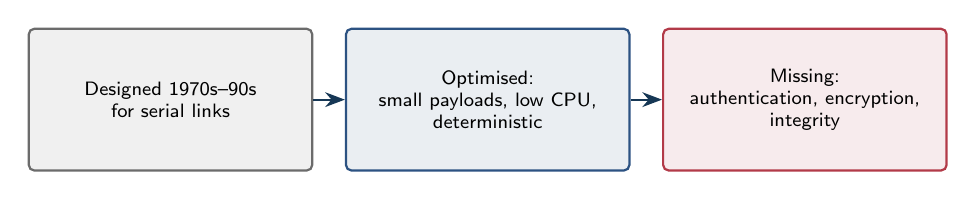
\begin{tikzpicture}[node distance=4mm]
  \node[isbox, fill=isMute!10, draw=isMute, minimum width=36mm, minimum height=18mm, align=center, font=\scriptsize] (then)
    {Designed 1970s--90s\\for serial links};
  \node[isbox, fill=isPLC!10, draw=isPLC, minimum width=36mm, minimum height=18mm, right=of then, align=center, font=\scriptsize] (req)
    {Optimised:\\small payloads, low CPU,\\deterministic};
  \node[isbox, fill=isAttack!10, draw=isAttack, minimum width=36mm, minimum height=18mm, right=of req, align=center, font=\scriptsize] (gap)
    {Missing:\\authentication, encryption,\\integrity};
  \draw[flow] (then) -- (req);
  \draw[flow] (req) -- (gap);
\end{tikzpicture}
\note{
  Set the framing before naming any single protocol: these wire formats predate routine internet use and were drawn for trusted serial loops where the physical layer \emph{was} the security boundary. Push back on the student reflex that ``newer = better'' --- the same Modbus frame from 1979 still runs in greenfield plants today because it is cheap, deterministic, and works. Misconception to flag early: ``but it runs over TCP now, so it must have TLS somewhere.'' No --- TCP only gives you a byte stream; it does not authenticate anything. Transition cue: ``so let us look at the canonical example, Modbus.''
}
\end{frame}

\section{Modbus}

\begin{frame}{Modbus Overview}
\centering
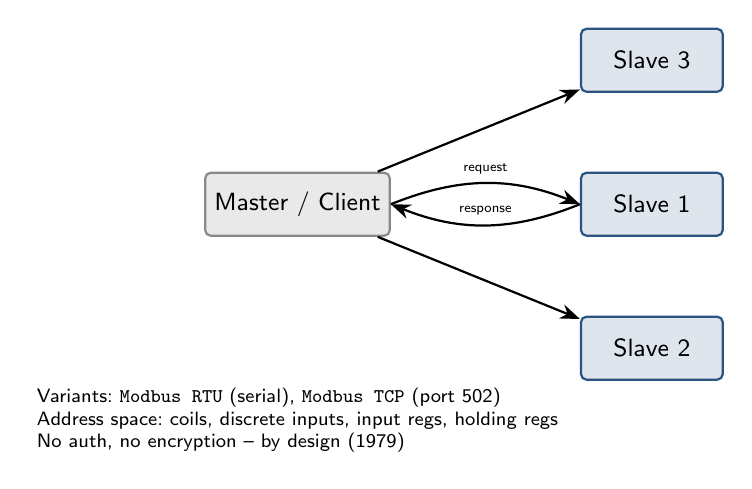
\begin{tikzpicture}[node distance=10mm]
  \node[server] (m) {Master / Client};
  \node[plc, right=24mm of m] (s1) {Slave 1};
  \node[plc, below=of s1] (s2) {Slave 2};
  \node[plc, above=of s1] (s3) {Slave 3};
  \draw[-{Stealth[length=2.5mm]}, thick] (m.east) to[bend left=22] node[midway, sloped, above=2pt, font=\tiny, fill=white, inner sep=1pt]{request} (s1.west);
  \draw[-{Stealth[length=2.5mm]}, thick] (s1.west) to[bend left=22] node[midway, sloped, above=2pt, font=\tiny, fill=white, inner sep=1pt]{response} (m.east);
  \draw[-{Stealth[length=2.5mm]}, thick] (m) -- (s2);
  \draw[-{Stealth[length=2.5mm]}, thick] (m) -- (s3);
  \node[font=\scriptsize, below=18mm of m, align=left]
    {Variants: \texttt{Modbus RTU} (serial), \texttt{Modbus TCP} (port 502)\\
     Address space: coils, discrete inputs, input regs, holding regs\\
     No auth, no encryption -- by design (1979)};
\end{tikzpicture}
\source{Modbus Organization, \emph{Modbus Application Protocol Specification} v1.1b3, 2012.}
\note{
  Anchor Modbus in time: it is older than ARP, older than DNS, older than most students in the room. The design assumption was a private 4-wire RS-485 loop on the shop floor, not the internet. When you see Modbus TCP today it is the original PDU with a 7-byte MBAP header bolted on --- function code intact, no auth, no integrity. Ask the room: ``Shodan shows tens of thousands of devices on port 502 --- what would you check first?'' Steer them toward unit-ID enumeration and function-code 8 (diagnostics) before anything destructive. Transition cue: ``let us decode an actual frame so you can read it on the wire.''
}
\end{frame}

\begin{frame}[fragile]{Modbus TCP Frame Anatomy}
\centering
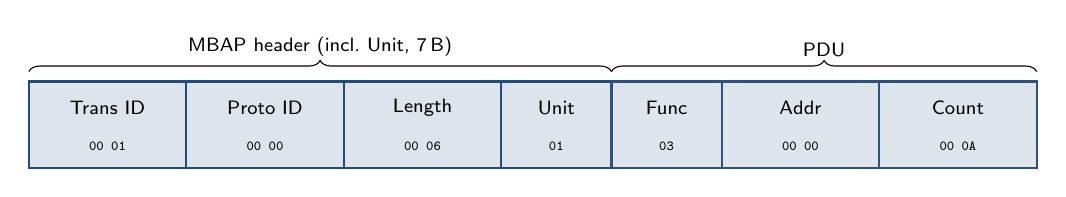
\begin{tikzpicture}[x=10mm, y=11mm, font=\scriptsize]
  \foreach \x/\w/\name/\hex/\col in {
    0/2/{Trans ID}/{00 01}/isOT,
    2/2/{Proto ID}/{00 00}/isOT,
    4/2/{Length}/{00 06}/isOT,
    6/1.4/{Unit}/{01}/isOT,
    7.4/1.4/{Func}/{03}/isPLC,
    8.8/2.0/{Addr}/{00 00}/isPLC,
    10.8/2.0/{Count}/{00 0A}/isPLC}{
    \draw[fill=\col!15, draw=\col, thick] (\x,0) rectangle ++(\w,1);
    \node[align=center] at (\x+\w/2,0.7) {\name};
    \node[font=\tiny\ttfamily, anchor=center] at (\x+\w/2,0.25) {\hex};
  }
  \draw[brace] (0,1.05) -- (7.4,1.05) node[midway,above=4pt]{MBAP header (incl.\ Unit, 7\,B)};
  \draw[brace] (7.4,1.05) -- (12.8,1.05) node[midway,above=4pt]{PDU};
\end{tikzpicture}
\vspace{4mm}
\begin{notebox}{Decoded}
``Read 10 holding registers starting at address \texttt{0x0000} from slave \texttt{1}.''
\end{notebox}
\note{
  Walk the bytes left-to-right at the board: transaction ID is a client-chosen correlation cookie, protocol ID is always zero for Modbus, length counts everything from the unit byte onward. Stress that the unit ID was originally the RS-485 slave address and is now reused as a gateway selector --- a single Modbus TCP endpoint can front a whole RTU bus. Common student misconception: they treat ``Function 03'' as read-only and therefore safe; remind them that Function 06 (single write) and 16 (multi-write) sit one byte away. Quick class question: ``what changes in this frame if we want to write coils instead of read registers?'' Answer: function code becomes 0x05 or 0x0F, plus a value field. Transition cue: ``Modbus is the simple case --- vendors like Siemens went their own way.''
}
\end{frame}

\section{Siemens, DNP3, EtherNet/IP}

\begin{frame}{Siemens S7comm}
\centering
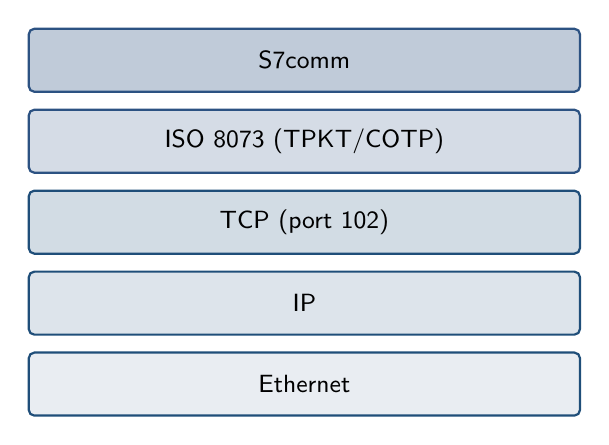
\begin{tikzpicture}[node distance=2mm]
  \node[isbox, fill=isOT!10, draw=isOT, minimum width=70mm, minimum height=8mm] (eth) {Ethernet};
  \node[isbox, fill=isOT!15, draw=isOT, minimum width=70mm, minimum height=8mm, above=of eth] (ip) {IP};
  \node[isbox, fill=isOT!20, draw=isOT, minimum width=70mm, minimum height=8mm, above=of ip] (tcp) {TCP (port 102)};
  \node[isbox, fill=isPLC!20, draw=isPLC, minimum width=70mm, minimum height=8mm, above=of tcp] (cotp) {ISO 8073 (TPKT/COTP)};
  \node[isbox, fill=isPLC!30, draw=isPLC, minimum width=70mm, minimum height=8mm, above=of cotp] (s7) {S7comm};
\end{tikzpicture}
\par\vspace{2mm}
\footnotesize Read/write variables, upload/download programs, start/stop CPU. S7commPlus added session keys -- still broken in practice.
\note{
  Walk up the stack from Ethernet to S7comm so students see why classic packet captures show TPKT/COTP framing first --- it is ISO transport over TCP because Siemens reused their pre-IP stack. The war story: S7comm has no authentication on classic S7-300/400, and the protocol was reverse-engineered well enough that Snap7 and python-snap7 give you full PLC control in a few lines. S7commPlus added an anti-replay handshake on S7-1200/1500, but researchers (Lei \emph{et al.}, Biham, Plc-blaster) showed the key material was derivable; Siemens has rotated it several times. Misconception: ``a firmware upgrade fixes it.'' Often the upgrade silently changes the wire format and breaks third-party tools without actually adding cryptographic identity. Transition cue: ``the utilities sector hit the same wall but answered differently.''
}
\end{frame}

\begin{frame}{DNP3 and IEC 60870-5-104}
\centering
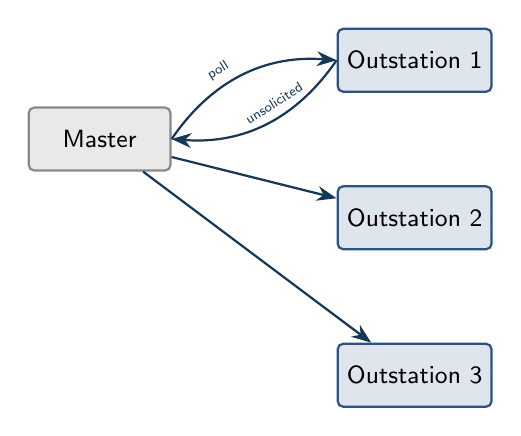
\begin{tikzpicture}[node distance=12mm]
  \node[server] (master) {Master};
  \node[plc] (out1) at (4,1) {Outstation 1};
  \node[plc] (out2) at (4,-1) {Outstation 2};
  \node[plc] (out3) at (4,-3) {Outstation 3};
  \draw[flow] (master.east) to[bend left=30] node[pos=0.4, sloped, above=2pt, font=\tiny, fill=white, inner sep=1pt]{poll} (out1.west);
  \draw[flow] (out1.west) to[bend left=30] node[pos=0.4, sloped, above=2pt, font=\tiny, fill=white, inner sep=1pt]{unsolicited} (master.east);
  \draw[flow] (master) -- (out2);
  \draw[flow] (master) -- (out3);
\end{tikzpicture}
\par\vspace{1mm}
{\footnotesize DNP3 dominant in NA utilities; IEC 60870-5-104 in Europe. Both ride TCP today; both added Secure Authentication (SAv5) on top, but encryption is optional.}
\source{IEEE 1815-2012 (DNP3) \textbar{} IEC 60870-5-104:2006 + Amd.\,1:2016.}
\note{
  Highlight the master/outstation model and the \emph{unsolicited response} pattern --- outstations push event data back without being polled, which is essential when a substation has a fault to report. War story: DNP3 SAv5 was standardised in IEEE 1815-2012 with HMAC-based challenge/response, and over a decade later real-world adoption in the field is still measured in single-digit percentages; utilities cite key-management overhead and the fact that the link layer is often a leased serial circuit they already trust. Misconception: ``SAv5 means encrypted.'' No --- it provides authentication only; confidentiality requires bump-in-the-wire TLS or IPsec. Class question: ``why might a utility leave SAv5 off even after they buy capable RTUs?'' Transition cue: ``Rockwell took yet another approach with EtherNet/IP.''
}
\end{frame}

\begin{frame}{EtherNet/IP and CIP}
\centering
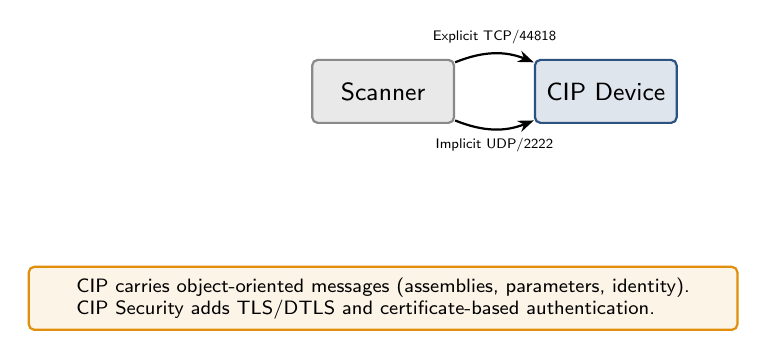
\begin{tikzpicture}[node distance=10mm]
  \node[server] (scan) {Scanner};
  \node[plc, right=of scan] (dev) {CIP Device};
  \draw[-{Stealth[length=2mm]}, thick] (scan) to[bend left=22] node[midway, sloped, above=2pt, font=\tiny, fill=white, inner sep=1pt]{Explicit TCP/44818} (dev);
  \draw[-{Stealth[length=2mm]}, thick] (scan) to[bend right=22] node[midway, sloped, below=2pt, font=\tiny, fill=white, inner sep=1pt]{Implicit UDP/2222} (dev);
  \node[isbox, fill=isAccent!10, draw=isAccent, below=18mm of scan, font=\scriptsize, align=left, minimum width=90mm]
    {CIP carries object-oriented messages (assemblies, parameters, identity).\\CIP Security adds TLS/DTLS and certificate-based authentication.};
\end{tikzpicture}
\note{
  Make the split explicit: \emph{explicit} messaging is request/response over TCP/44818 for configuration and diagnostics; \emph{implicit} (a.k.a.\ I/O) is cyclic UDP/2222 multicast for the actual control data --- which is why blocking 44818 alone does not stop a running line. CIP itself is an object model; EtherNet/IP is just CIP-over-Ethernet. War story: ODVA standardised CIP Security in 2015 with TLS for explicit and DTLS for implicit traffic, but Rockwell only ships it on newer ControlLogix 5580 / CompactLogix 5380 firmware, and rolling certificates across hundreds of drives is a project few sites have funded. Misconception: ``EtherNet/IP is just industrial Ethernet.'' No --- the name is a marketing collision; it is CIP encapsulated in Ethernet frames, nothing to do with the EtherNet trademark. Transition cue: ``Siemens did the same idea differently with Profinet.''
}
\end{frame}

\begin{frame}{Profinet}
\centering
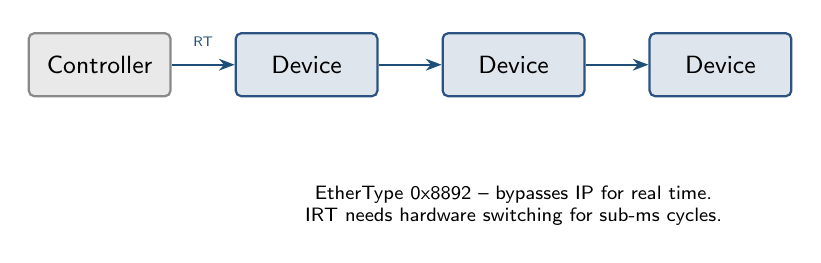
\begin{tikzpicture}[node distance=8mm]
  \node[server] (ctl) {Controller};
  \node[plc, right=of ctl] (dev1) {Device};
  \node[plc, right=of dev1] (dev2) {Device};
  \node[plc, right=of dev2] (dev3) {Device};
  \draw[-{Stealth[length=2mm]}, thick, isOT] (ctl) -- node[midway, above, font=\tiny, yshift=1mm]{RT} (dev1);
  \draw[-{Stealth[length=2mm]}, thick, isOT] (dev1) -- (dev2);
  \draw[-{Stealth[length=2mm]}, thick, isOT] (dev2) -- (dev3);
  \node[font=\scriptsize, below=10mm of dev2, align=center]
    {EtherType 0x8892 -- bypasses IP for real time.\\IRT needs hardware switching for sub-ms cycles.};
\end{tikzpicture}
\note{
  Stress that Profinet RT lives at layer 2 --- EtherType 0x8892, no IP, no TCP --- specifically because the IP stack adds jitter that breaks deterministic cycles. Profinet IRT goes further and requires switches with hardware time-slotting (typically IEEE 1588 PTP) for sub-millisecond updates. Security war story: Profinet has long-standing weaknesses around DCP (Discovery and Configuration Protocol), which lets anyone on the local segment rename or reset a device; multiple advisories (CERT@VDE, Claroty's OT:ICEFALL set in 2022) catalogued this. Misconception: ``it is layer 2 so it cannot be attacked remotely.'' True --- but most Profinet networks share VLANs with the engineering laptops, and a compromised laptop is on the wire. Transition cue: ``so what does a protocol look like when security is designed in from day one?''
}
\end{frame}

\section{Modern Secure Protocols}

\begin{frame}{OPC UA}
\centering
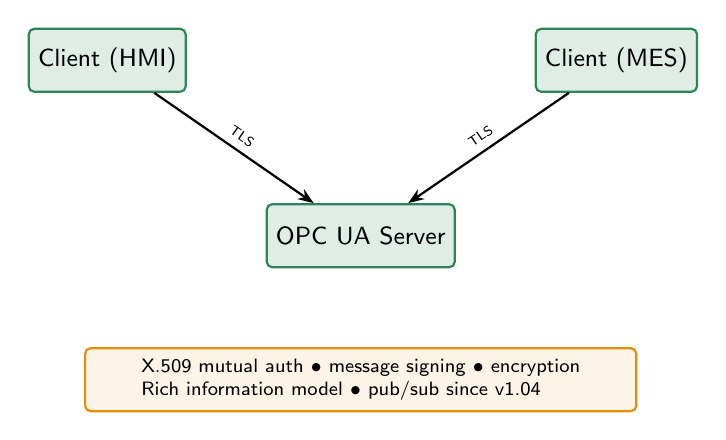
\begin{tikzpicture}[node distance=10mm]
  \node[server, fill=isHMI!15, draw=isHMI] (srv) {OPC UA Server};
  \node[hmi, above left=14mm and 10mm of srv] (c1) {Client (HMI)};
  \node[hmi, above right=14mm and 10mm of srv] (c2) {Client (MES)};
  \node[isbox, fill=isAccent!10, draw=isAccent, below=of srv, font=\scriptsize, minimum width=70mm, align=left]
    {X.509 mutual auth $\bullet$ message signing $\bullet$ encryption\\Rich information model $\bullet$ pub/sub since v1.04};
  \draw[-{Stealth[length=2mm]}, thick] (c1) -- node[midway, sloped, above=2pt, font=\tiny, fill=white, inner sep=1pt]{TLS} (srv);
  \draw[-{Stealth[length=2mm]}, thick] (c2) -- node[midway, sloped, above=2pt, font=\tiny, fill=white, inner sep=1pt]{TLS} (srv);
\end{tikzpicture}
\source{IEC 62541 (multipart, OPC Foundation) \textbar{} OPC UA Specification Part 2 (Security Model).}
\note{
  Sell OPC UA as the ``protocol with seatbelts'' --- mutual X.509 authentication, signed messages, optional encryption, and a rich information model that lets you discover what a device \emph{is}, not just what registers it has. Critical war story: the specification is over a dozen parts and a thousand pages; surveys (e.g.\ Kaspersky ICS-CERT, Claroty Team82 ``OPC UA Deep Dive'') repeatedly find that a large share of real-world deployments run with security policy ``None'' and anonymous user tokens because that is the default in many configurators. Misconception: ``OPC UA always uses TLS.'' No --- the binary transport has its own message-level crypto, and you must explicitly pick a SecurityPolicy like \texttt{Basic256Sha256} or \texttt{Aes256\_Sha256\_RsaPss}; ``None'' is a valid choice. Class question: ``how would you audit a plant to find anonymous-mode OPC UA servers?'' Transition cue: ``OPC UA is heavy --- MQTT is the lighter modern option.''
}
\end{frame}

\begin{frame}{MQTT for IIoT}
\centering
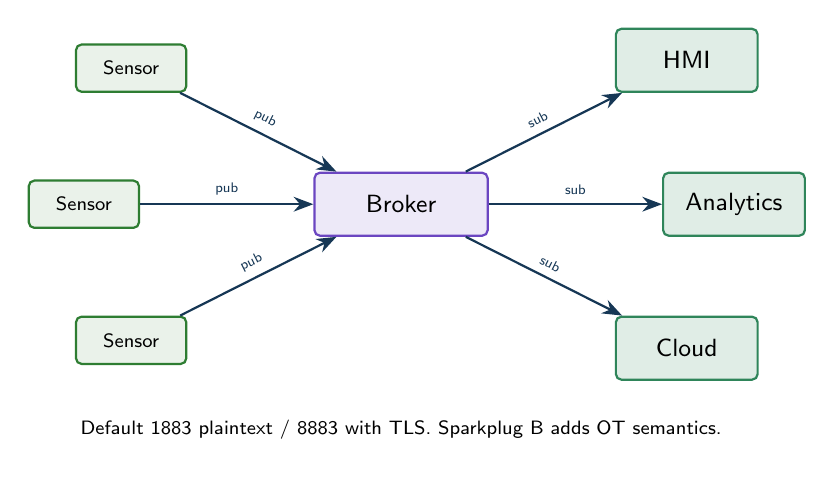
\begin{tikzpicture}[node distance=10mm]
  \node[server, fill=isSCADA!12, draw=isSCADA, minimum width=22mm] (br) {Broker};
  \node[sensor, above left=10mm and 16mm of br] (s1) {Sensor};
  \node[sensor, left=22mm of br] (s2) {Sensor};
  \node[sensor, below left=10mm and 16mm of br] (s3) {Sensor};
  \node[hmi, above right=10mm and 16mm of br] (sub1) {HMI};
  \node[hmi, right=22mm of br] (sub2) {Analytics};
  \node[hmi, below right=10mm and 16mm of br] (sub3) {Cloud};
  \foreach \n in {s1,s2,s3}{\draw[flow] (\n) -- node[midway, sloped, above=2pt, font=\tiny, fill=white, inner sep=1pt]{pub} (br);}
  \foreach \n in {sub1,sub2,sub3}{\draw[flow] (br) -- node[midway, sloped, above=2pt, font=\tiny, fill=white, inner sep=1pt]{sub} (\n);}
  \node[font=\scriptsize, below=22mm of br] {Default 1883 plaintext / 8883 with TLS. Sparkplug B adds OT semantics.};
\end{tikzpicture}
\note{
  Frame MQTT as the publish/subscribe answer for IIoT: the broker is the choke point, sensors publish topics, anything authorised subscribes. Note the two ports --- 1883 plaintext and 8883 with TLS --- and remind students that Shodan finds hundreds of thousands of brokers on 1883 with no authentication and \texttt{\#} wildcard subscriptions open. War story: in 2018 Avast scanned the open MQTT space and found brokers leaking smart-home, prison, and industrial telemetry; the situation has improved but not vanished. Sparkplug B (Eclipse Foundation) is worth mentioning because it adds the OT semantics MQTT lacks --- state, birth/death certificates, structured payloads --- and it is what most modern Unified Namespace deployments use. Misconception: ``MQTT 5 is encrypted by default.'' No --- MQTT 5 added user properties and better error codes, not transport security; you still need TLS underneath. Transition cue: ``let us put everything side by side.''
}
\end{frame}

\begin{frame}{Protocol Security at a Glance}
\centering
\renewcommand{\arraystretch}{1.3}
\footnotesize
\begin{tabular}{|l|c|c|c|l|}
\hline
\rowcolor{isMute!20}
\textbf{Protocol} & \textbf{Auth} & \textbf{Integrity} & \textbf{Confid.} & \textbf{Notes} \\
\hline
Modbus       & \cellcolor{isAttack!20}$\times$ & \cellcolor{isAttack!20}$\times$ & \cellcolor{isAttack!20}$\times$ & 1979, ubiquitous \\
S7comm       & \cellcolor{isAttack!20}$\times$ & \cellcolor{isAttack!20}$\times$ & \cellcolor{isAttack!20}$\times$ & Siemens-proprietary \\
DNP3         & \cellcolor{isAccent!20}opt SAv5 & \cellcolor{isAccent!20}opt     & \cellcolor{isAttack!20}$\times$ & Utilities \\
EtherNet/IP  & \cellcolor{isAccent!20}opt CIP  & \cellcolor{isAccent!20}opt     & \cellcolor{isAccent!20}opt      & Rockwell \\
Profinet     & \cellcolor{isAttack!20}weak     & \cellcolor{isAttack!20}$\times$ & \cellcolor{isAttack!20}$\times$ & Siemens / IRT \\
OPC UA       & \cellcolor{isNet!25}X.509       & \cellcolor{isNet!25}sign       & \cellcolor{isNet!25}TLS         & modern default \\
MQTT         & \cellcolor{isAccent!20}+TLS     & \cellcolor{isNet!25}TLS         & \cellcolor{isNet!25}TLS         & IIoT messaging \\
\hline
\end{tabular}
\note{
  Use the table to make a single argument: the security column is mostly a story about \emph{defaults}. The protocols marked ``opt'' (DNP3 SAv5, CIP Security, MQTT+TLS) technically support strong crypto, but the boxes ship without it and the engineers configuring them rarely turn it on. Only OPC UA was designed with a non-trivial default --- and even then operators routinely downgrade to SecurityPolicy ``None'' to fix interoperability. Misconception to puncture: ``the green cells are safe protocols.'' No, they are protocols where safety is possible; whether you got it depends on the deployment. Ask the class: ``of these seven, which one would you put on a new greenfield project and why?'' --- there is no single right answer, the trade-off is determinism vs.\ security vs.\ ecosystem. Transition cue: ``one application area pushes all of this to extremes --- substations.''
}
\end{frame}

\begin{frame}{IEC 61850 in Substations}
\centering
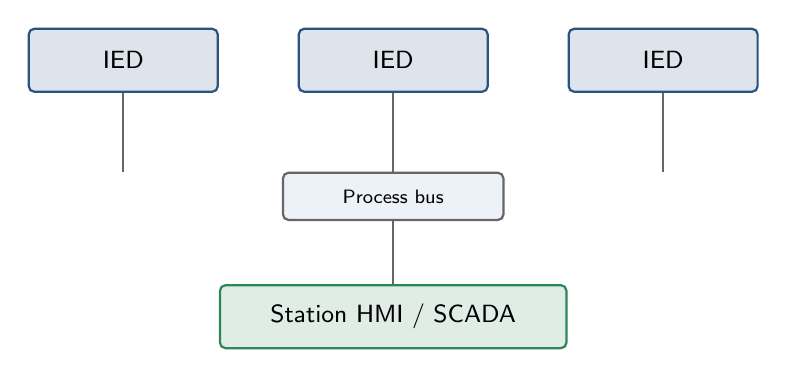
\begin{tikzpicture}[node distance=10mm]
  \node[plc, fill=isOT!15, minimum width=24mm] (ied1) {IED};
  \node[plc, fill=isOT!15, minimum width=24mm, right=of ied1] (ied2) {IED};
  \node[plc, fill=isOT!15, minimum width=24mm, right=of ied2] (ied3) {IED};
  \node[switch, below=10mm of ied2, minimum width=28mm] (sw) {Process bus};
  \node[server, fill=isHMI!15, draw=isHMI, below=8mm of sw, minimum width=44mm, font=\small] (scada) {Station HMI / SCADA};
  \draw[netline] (ied1.south) -- (ied1.south |- sw.north);
  \draw[netline] (ied2.south) -- (sw.north);
  \draw[netline] (ied3.south) -- (ied3.south |- sw.north);
  \draw[netline] (sw.south) -- (scada.north);
\end{tikzpicture}
\vspace{1mm}
\begin{notebox}{The substation stack}
\textbf{MMS} for client/server; \textbf{GOOSE} for sub-4\,ms trip messages; \textbf{Sampled Values} for measurements. Goose has \emph{no} authentication by default.
\end{notebox}
\source{IEC 61850 (multipart) \textbar{} IEC 62351 (security for IEC TC 57 protocols).}
\note{
  Walk through the three services in order of latency budget: MMS for slow client/server, GOOSE for fast trip and interlock signals (layer 2 multicast, target end-to-end under 4\,ms), and Sampled Values streaming raw current and voltage at the sampling rate of the merging unit. War story: a spoofed GOOSE frame can trip a breaker because the receiver only checks the state number and sequence; this exact attack family was demonstrated by Hoyos \emph{et al.}\ and later operationalised by the CRASHOVERRIDE/Industroyer malware against the Ukrainian grid in 2016. IEC 62351-6 specifies authentication for GOOSE and SV, but few merging units actually implement it and switching it on adds latency the protection engineer may not tolerate. Misconception: ``GOOSE is just multicast Ethernet, not a security concern.'' It is exactly the lack of crypto on a high-trust safety bus that makes it interesting. Transition cue: ``let us pull the section together.''
}
\end{frame}

\begin{frame}{Summary -- Section \sectionNumber}
\begin{takeawaybox}{What to remember from this section}
\begin{itemize}\setlength{\itemsep}{2pt}
  \item Most legacy industrial protocols are unauthenticated and unencrypted by design.
  \item Modbus is the canonical example -- 12 bytes of MBAP and a one-byte function code.
  \item Modern protocols (OPC UA, MQTT-TLS) bring real cryptography, but require correct configuration.
  \item Network-layer mitigations (firewalls, segmentation) compensate where the protocol cannot.
\end{itemize}
\end{takeawaybox}
\note{
  Land the section on one sentence: the protocol layer almost never gives you the security you want, so the compensating controls live in the network and in the process. Reinforce the Modbus number --- 7-byte MBAP plus a one-byte function code is enough to read or write any register in any device on a bus, and that is the threat model most students will meet in their first OT engagement. Flag that the next section moves from \emph{what is on the wire} to \emph{how to put up walls around the wire}: firewalls, conduits, the Purdue model. If there is time, take one question on which protocol surprised them most --- it is usually OPC UA, because the gap between specification and default deployment is the largest.
}
\end{frame}

\referencesframe{
  \item Modbus Organization. \emph{Modbus Application Protocol Specification} v1.1b3, 2012.
  \item Modbus Organization. \emph{Modbus/TCP Security}, 2018.
  \item IEEE 1815-2012. \emph{Electric Power Systems Communications -- DNP3}.
  \item IEC 60870-5-104:2006 + Amd.\,1:2016. \emph{Telecontrol equipment -- Network access for IEC 60870-5-101}.
  \item IEC 62541 (multipart). \emph{OPC Unified Architecture} (OPC Foundation).
  \item IEC 61850 (multipart). \emph{Communication networks and systems for power utility automation}.
  \item IEC 62351 (multipart). \emph{Security for TC 57 protocols}.
  \item OASIS. \emph{MQTT Version 5.0}, 2019.
  \item ODVA. \emph{The CIP Networks Library, Volume 1-8}, CIP Security spec.
  \item Siemens. \emph{Step7 \& S7 communication protocols} (S7comm, S7commPlus).
  \item Wightman, R. \emph{Project Basecamp -- ICS Vulnerability Catalog}, Digital Bond, 2012.
}

\closingframe

\end{document}
